\newpage
\subsection{Transaction}

\ifbook{

  \paragraph{} La plupart des applications en ligne ont généralement comme objectif de réaliser des
  \textbf{transactions}. On mesure d'ailleurs très souvent la performance d'un système au nombre de
  transactions effectuées par minute. La notion de transaction est donc au coeur de bien des aspects
  du \textbf{middleware}.

  \paragraph{} Bien que l'usage du terme \textbf{transaction} soit très répandu, son sens n'est
  forcément aussi clairement maitrisé. Nous allons commencer par étudier sa définition. D'après
  \mylink{http://fr.wikipedia.org/wiki/Transaction\_informatique}{Wikipédia} la définition d'une
  transaction (accédée le 27/12/2011) est la suivante:

  \paragraph{} \textit{En informatique, et particulièrement dans les bases de données, une
  transaction telle qu'une réservation, un achat ou un paiement est mise en oeuvre via une suite
  d'opérations qui font passer la base de données d'un état A - antérieur à la transaction - à un
  état B postérieur et des mécanismes permettent d'obtenir que cette suite soit à la fois atomique,
  cohérente, isolée et durable (ACID):}

  \begin{description}
    \item[atomique] \textit{la suite d'opérations est indivisible, en cas d'échec en cours d'une des
    opérations, la suite d'opérations doit être complètement annulée (rollback) quel que soit le
    nombre d'opérations déjà réussies.}
    \item[cohérente] \textit{le contenu de la base de données à la fin de la transaction doit être
    cohérent sans pour autant que chaque opération durant la transaction donne un contenu cohérent.
    Un contenu final incohérent doit entraîner l'échec et l'annulation de toutes opérations de la
    transaction.}
    \item[isolée] \textit{lorsque deux transactions A et B sont exécutées en même temps, les
    modifications effectuées par A ne sont ni visibles par B, ni modifiables par B tant que la
    transaction A n'est pas terminée et validée (commit).}
    \item[durable] \textit{Une fois validé, l'état de la base de données doit être permanent, et
    aucun incident technique (exemple: crash) ne doit pouvoir engendrer une annulation des
    opérations effectuées durant la transaction.}
  \end{description}

  \begin{figure}[hb]
    \begin{center}
      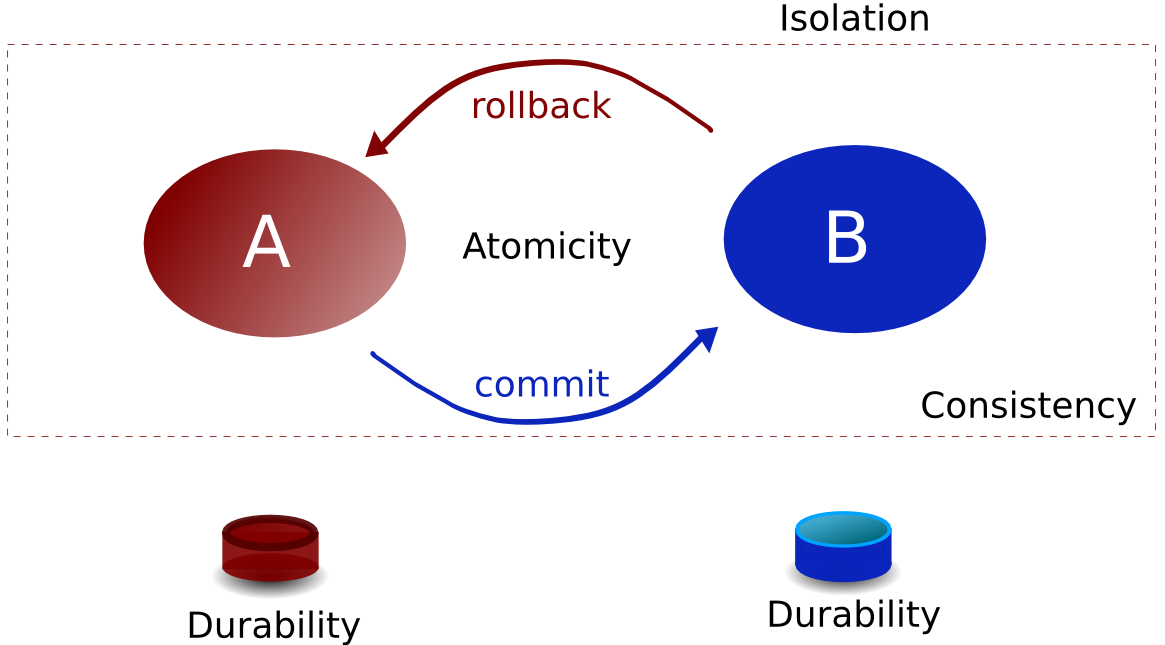
\includegraphics[scale=0.4]{img/transaction.png}
      \caption{Caractéristique d'une transaction}
      \label{tx}
    \end{center}
  \end{figure}
}

\ifslide{
  \begin{frame}{Transaction}
   \begin{center}
     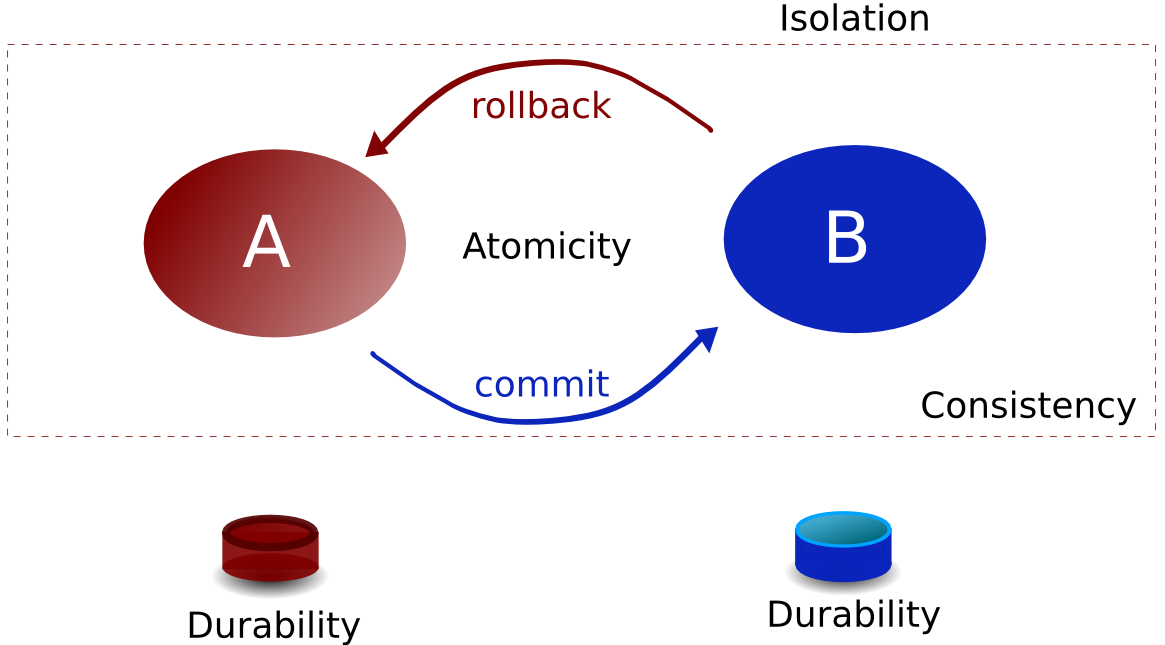
\includegraphics[scale=0.3]{img/transaction.png}
   \end{center}
  \end{frame}
}


%- Compensating transaction
